%%%%%%%%%%%%%%%%%%%%%%%%%%%%%%%%%%%%%%%%%%%%%%%%%%%%%%%%%%%%%%%%%%%%%%%%%%%%%%%%%%%%%%%%%%%%%%%%
%
% CS484 Written Question Template
%
% Acknowledgements:
% The original code is written by Prof. James Tompkin (james_tompkin@brown.edu).
% The second version is revised by Prof. Min H. Kim (minhkim@kaist.ac.kr).
%
% This is a LaTeX document. LaTeX is a markup language for producing 
% documents. Your task is to fill out this document, then to compile 
% it into a PDF document. 
%
% 
% TO COMPILE:
% > pdflatex thisfile.tex
%
% If you do not have LaTeX and need a LaTeX distribution:
% - Personal laptops (all common OS): www.latex-project.org/get/
% - We recommend latex compiler miktex (https://miktex.org/) for windows,
%   macTex (http://www.tug.org/mactex/) for macOS users.
%   And TeXstudio(http://www.texstudio.org/) for latex editor.
%   You should install both compiler and editor for editing latex.
%   The another option is Overleaf (https://www.overleaf.com/) which is 
%   an online latex editor.
%
% If you need help with LaTeX, please come to office hours. 
% Or, there is plenty of help online:
% https://en.wikibooks.org/wiki/LaTeX
%
% Good luck!
% Min and the CS484 staff
%
%%%%%%%%%%%%%%%%%%%%%%%%%%%%%%%%%%%%%%%%%%%%%%%%%%%%%%%%%%%%%%%%%%%%%%%%%%%%%%%%%%%%%%%%%%%%%%%%
%
% How to include two graphics on the same line:
% 
% \includegraphics[\width=0.49\linewidth]{yourgraphic1.png}
% \includegraphics[\width=0.49\linewidth]{yourgraphic2.png}
%
% How to include equations:
%
% \begin{equation}
% y = mx+c
% \end{equation}
% 
%%%%%%%%%%%%%%%%%%%%%%%%%%%%%%%%%%%%%%%%%%%%%%%%%%%%%%%%%%%%%%%%%%%%%%%%%%%%%%%%%%%%%%%%%%%%%%%%

\documentclass[11pt]{article}

\usepackage[english]{babel}
\usepackage[utf8]{inputenc}
\usepackage[colorlinks = true,
            linkcolor = blue,
            urlcolor  = blue]{hyperref}
\usepackage[a4paper,margin=1.5in]{geometry}
\usepackage{stackengine,graphicx}
\usepackage{fancyhdr}
\setlength{\headheight}{15pt}
\usepackage{microtype}
\usepackage{times}
\usepackage{booktabs}

% From https://ctan.org/pkg/matlab-prettifier
\usepackage[numbered,framed]{matlab-prettifier}

\frenchspacing
\setlength{\parindent}{0cm} % Default is 15pt.
\setlength{\parskip}{0.3cm plus1mm minus1mm}

\pagestyle{fancy}
\fancyhf{}
\lhead{Homework Writeup}
\rhead{CS484}
\rfoot{\thepage}

\date{}

\title{\vspace{-1cm}Homework 5 Writeup}


\begin{document}
\maketitle
\vspace{-3cm}
\thispagestyle{fancy}

\section*{Instructions}
\begin{itemize}
  \item Describe any interesting decisions you made to write your algorithm.
  \item Show and discuss the results of your algorithm.
  \item Feel free to include code snippets, images, and equations.
  \item Use as many pages as you need, but err on the short side If you feel you only need to write a short amount to meet the brief, th
  
  \item \textbf{Please make this document anonymous.}
\end{itemize}

\section*{In the beginning...}

I implement the Scene Recognition with 3 methods:
\begin{enumerate}
    \item tiny images + nearest neighbor
    \item bag of words (bow) + nearest neighbor
    \item bag of words (bow) + one vs. all linear SVM
\end{enumerate}

\section*{Interesting Implementation Detail}

- tiny images

Here, I use image as a feature itself. Get a image, resize to 16x16, reshape to 1x256 vector and normalize. Please refer the code.
\begin{lstlisting}[style=Matlab-editor]
for i=1:n
    image = im2double(imread(image_paths{i}));
    image = imresize(image, [16 16]);
    image = reshape(image, 1, 256);
    image = image - mean(image);
    image = image./norm(image);
    image_feats(i,:) = image;
end
\end{lstlisting}

- nearest neighbor classify

Here, I implement the 1 nearest neighbor. Calculate the L2 distance by pdist2() between train and test feature set, and find the most closest feature. Please refer the code.
\begin{lstlisting}[style=Matlab-editor]
n = size(test_image_feats, 1);
predicted_categories = cell(n, 1);
D = pdist2(train_image_feats, test_image_feats);
for i = 1:n
    D_i = D(:,i);
    [~, idx] = min(D_i);
    predicted_categories(i) = train_labels(idx);
end
\end{lstlisting}

- build vocabulary

Here, we build vocabulary for bow. Using meshgrid() and extractHOGFeatures(), I extract features at every 20x20 grid points using CellSize 16x16. Then using kmeans cluster the features. For calculation speed, I choose random samples from image data using randperm(). Please refer the code.
\begin{lstlisting}[style=Matlab-editor]
n = size(image_paths,1);
r = 0.1;
x = 1:20:256;
y = 1:20:256;
[X, Y] = meshgrid(x, y);
X = reshape(X, [], 1);
Y = reshape(Y, [], 1);
results = [];
sample = randperm(n, floor(n*r)); %random sampling from images

for i=sample
    image = imread(image_paths{i});
    features = extractHOGFeatures(image, [X Y], 'CellSize', [16 16]);
    results = cat(1, results, features);
end
[~, vocab] = kmeans(results, vocab_size);
\end{lstlisting}

- get bags of words

Here, using the vocabulary above, get the images' histograms. First, extract the image's SIFT features. Then, find the most closest feature in the vocabulary 'vocab' for each features. The histogram is used for image's feature for classification. Please refer the code.
\begin{lstlisting}[style=Matlab-editor]
for i=1:N
    hgram = zeros(1, vocab_size);
    image = imread(image_paths{i});
    features = extractHOGFeatures(image, [X Y], 'CellSize', [16 16]);
    D = pdist2(features, vocab);
    features_size = size(D, 1);
    for j=1:features_size
        [~, idx] = min(D(j,:));
        hgram(1, idx) = hgram(1, idx) + 1;
    end
    hgram = hgram/norm(hgram);
    image_feats(i,:) = hgram;
end
\end{lstlisting}

- SVM classify

Finally, here I implement the svm classifier. For training one vs all model, make a label by strcmp() and set the non-target class label values to -1. With fitclinear(), make a SVM one vs all model. Using the model, predict the image's class with predict(). Find the most confident class. Please refer the code.
\begin{lstlisting}[style=Matlab-editor]
for i=1:num_categories
    mask = strcmp(categories(i), train_labels);
    label = double(mask);
    label(~mask) = -1;
    Mdl = fitclinear(train_image_feats, label, 'Lambda', Lambda);
    [labelIdx, score] = predict(Mdl, test_image_feats);
    confidences(:,i) = score(:,2);
end
[~, idx] = max(confidences, [], 2);
predicted_categories = categories(idx);
\end{lstlisting}
\section*{A Result}

\begin{enumerate}
    \item Case1: tiny images + nearest neighbor (Figure~\ref{fig:result1}). Show the shortest time and lowest accuracy, because the simplest methods are used.
    \item Case2: bag of words (bow) + nearest neighbor (Figure~\ref{fig:result2}). It takes the most time and accuracy is improved than case1. It means the bag of words is better than simple image. 
    \item Case3: bag of words (bow) + one vs. all linear SVM (Figure~\ref{fig:result3}). It takes time similar with 2 and shows the highest accuracy due to bow and SVM. 
\end{enumerate}

\begin{figure}[h]
    \centering
    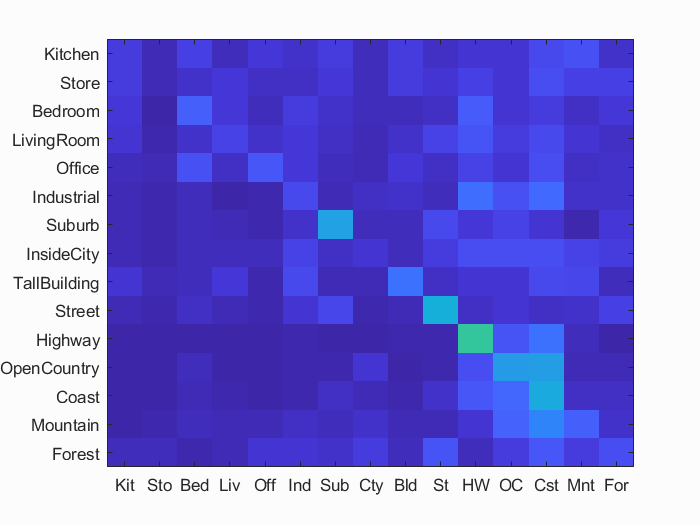
\includegraphics[width=13cm]{writeup/confusion_matrix1.png}
    \caption{confusion matrix for case1}
    \label{fig:result1}
\end{figure}
\begin{figure}[h]
    \centering
    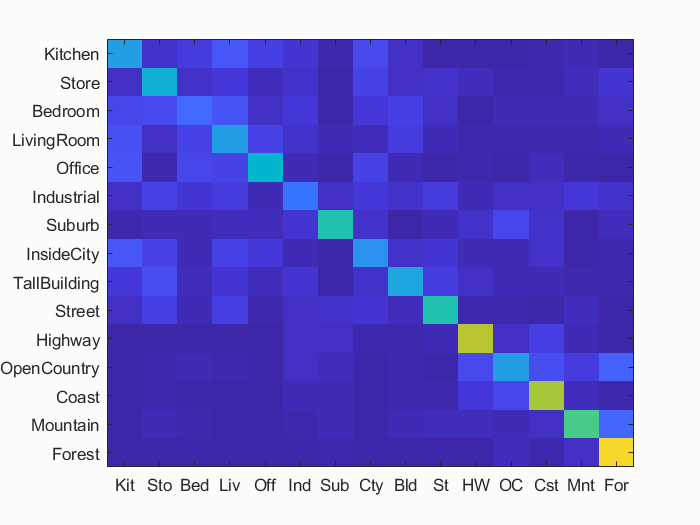
\includegraphics[width=13cm]{writeup/confusion_matrix2.png}
    \caption{confusion matrix for case2}
    \label{fig:result2}
\end{figure}
\begin{figure}[h]
    \centering
    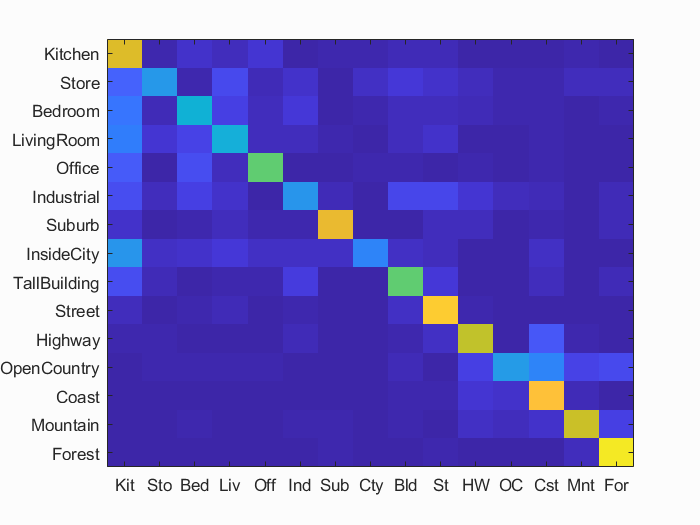
\includegraphics[width=13cm]{writeup/confusion_matrix3.png}
    \caption{confusion matrix for case3}
    \label{fig:result3}
\end{figure}

My results are summarized in Table~\ref{tab:table1}.

\begin{table}[h]
    \centering
    \begin{tabular}{lrr}
        \toprule
        Condition & Time (seconds) & accuracy\\
        \midrule
        Case 1 & 13.108 & 0.224\\
        Case 2 & 314.842 & 0.474\\
        Case 3 & 260.234 & 0.611\\
        \bottomrule
    \end{tabular}
    \caption{Result of 3 cases}
    \label{tab:table1}
\end{table}

\end{document}
